\chapter{Data Preprocessing}
\label{ch:data-preprocessing}

\begin{figure}
    \centering
    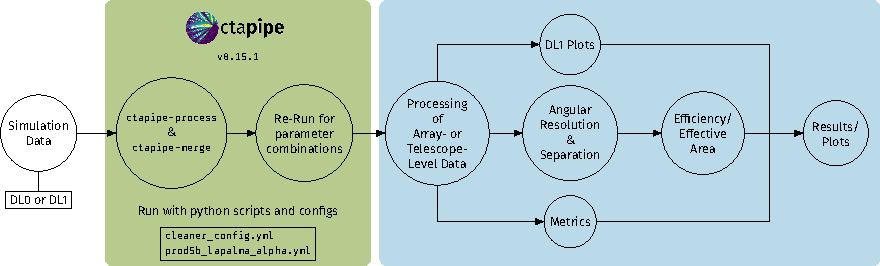
\includegraphics[width=\textwidth]{graphics/data_pipeline.pdf}
    \caption{Data Preprocessing}
    \label{fig:data-preprocessing}
\end{figure}

\begin{minipage}{\textwidth}
  \begin{mdframed}[backgroundcolor=white!20!black,leftmargin=0cm,rightmargin=0cm, skipabove=0pt, innerleftmargin=0,innerrightmargin=0,]
  \begin{pythonlst}
    def metrics(events, output_file_metrics, unique_file_id):
        """Calculates the metrics for the given telescope type.

        Parameters:
        -----------
        events: astropy.table.Table
            The events table. Must contain the following columns:
            - true_image: The true image of the event.
            - image: The event image containing background noise.
        output_file_metrics: pathlib.Path
            The path to the output file for the metrics.
        unique_file_id: int
            The unique file id for the input file.
        """

        # initialize the metrics calculator
        metrics_calc = TprFprCalculator(
            true_image=events["true_image"],
            image=events["image"],
            clean_mask=events["image_mask"]
        )

        # calculate the metrics
        metrics_data = metrics_calc.tpr_fpr()

        # write metrics data to DataFrame and then to a file
        metrics = pd.DataFrame(data=metrics_data)
        metrics.insert(loc=0, column='unique_file_id', value=unique_file_id)
        metrics.to_csv(
            output_file_metrics,
            index=False,
            mode='a',
            header=not output_file_metrics.exists()
        )
  \end{pythonlst}
  \end{mdframed}
\end{minipage}

